\chapter{\kadaib}
\section{\purpose}
今回の実験では,探索時間を指標とした視覚探索課題の心理物理実験をする.
心理物理実験とは,物理的世界に属する刺激強度と,心理的世界に属する感覚強度の数学的関数関係を明らかにする実験である\cite{心理物理測定法}.
今回は,視覚探索課題に対して心理物理実験をする.視覚探索課題とは,複数の刺激項目に対して,あらかじめ決められた目標項目があるか否かを,実験参加者が判断する課題である\cite{視覚探索}.
複数の刺激「妨害刺激」の中に,1つだけ異なる刺激「目標刺激」が存在する場合と,そうでない場合について,刺激数に対する探索時間を計測する.
実験参加者は,目標刺激が妨害刺激の中にあるかないかを,できるだけ早くかつ正確に判断する必要がある.\par
また,結果に対して統計的仮説検定をする.統計的仮説検定とは,標本を使って母集団に関する統計的な判断を下す方法である\cite[p.200]{Pythonで学ぶあたらしい統計学の教科書}.
探索時間が限りなく\(0\)になる「ポップアウト」,刺激数と探索時間が比例する「逐次探索(系列探索)」についての研究\cite{視覚探索課題と注意に関する研究動向}で,刺激種類と探索時間の関係について言及されている.
今回は\(t\)検定を用いて,視覚探索課題における探索非対称性\footnote{目標刺激と妨害刺激が交代しただけで,探索時間が非常に異なる現象のこと\cite{4視覚探索}.}があるか検討する.仮説は「探索非対称性がある」とし,仮説が正しい場合,目標刺激が異なる2条件に対して回帰直線の傾きに差が生じることを確認する.
その結果を踏まえて,刺激の種類と「ポップアウト」,「逐次探索」の関係について考察する.
\section{\method}
\paragraph{実験装置}
視覚探索課題の心理物理実験には,\matlab とPsychtoolbox を用いる.Psychtoolboxは,プログラミングを簡便にするツールであり,心理物理学の実験でよく用いられる.
データ分析するソフトウェアには\matlab とデータを集計するGoogleスプレットシートを用いる.
\begin{table}[H]
    \caption{実験装置\ (\kadaib)}
    \label{tbl:実験装置\kadaib}
    \begin{tabularx}{\textwidth}{cAR}
        \hline
        \multirow{5}{*}{\bfseries 刺激呈示コンピュータ}  & プロセッサ                    & Intel(R) Xeon(R) Gold 5218R CPU @ 2.10GHz     \\
                                               & メモリ                      & 11.7GB                                        \\
                                               & OS                       & Microsoft Windows 10 Enterprise LTSC 64bit    \\
                                               & \matlab                  & R2020b - academic use                         \\
                                               & Psychtoolbox             & バージョン不明                                       \\
        \hline
        \multirow{6}{*}{\bfseries データ分析コンピュータ} & コンピュータ                   & MacBook Air 2022 (Apple社)\texttt{MLY13J/A}    \\
                                               & プロセッサ                    & Apple Silicon M2\ \  8コアCPU,8コアGPU            \\
                                               & メモリ                      & 8GB                                           \\
                                               & OS                       & macOS 13.4                                    \\
                                               & \multirow{2}{*}{\matlab} & R2023a - academic use (Update1 9.14.02239454) \\
                                               &                          & 64-bit (maci64) March 30, 2023                \\
        \hline
    \end{tabularx}
\end{table}
\clearpage
\paragraph{視覚探索課題の心理物理実験}
以下に視覚探索課題の心理物理実験方法を示す.

\begin{wrapfigure}{r}[0mm]{.3\textwidth}
    \vspace{-1cm}
    \centering
    \input{sigeki}
    \caption{刺激対1}
    \label{fig:刺激対1}
    \begin{minipage}[t]{.13\textwidth}
        \centering
        \includegraphics[keepaspectratio,width=\textwidth]{../../13_BehavioralExperiment/syuri.png}
    \end{minipage}
    \begin{minipage}[t]{.13\textwidth}
        \centering
        \includegraphics[keepaspectratio,width=\textwidth]{../../13_BehavioralExperiment/star.png}
    \end{minipage}
    \caption{刺激対2\ \((40\times 40\textrm{pixel})\)}
    \label{fig:刺激対2}
    \vspace{-1cm}
\end{wrapfigure}
\noindent\textbf{\underline{<実験1>}}(\sref{src:13_01},\sref{src:13_02})
\begin{enumerate}
    \renewcommand{\labelenumi}{\fbox{\theenumi}}
    \item 注視点が\(500\textrm{ms}\)表示される.
    \item 画面に刺激(刺激対1:\figref{fig:刺激対1})が表示される.画面に表示される合計の刺激数は\(4,8,16\)個のいずれかである.円の刺激を\texttt{C},円と棒の刺激を\texttt{CL}とする.刺激の大きさは,\(40\times40\textrm{pixel}\)とする.
    \item 目標刺激が妨害刺激の中にある場合はキーボード上「\texttt{F}」,そうでない場合は「\texttt{J}」を押下し\ \fbox{1}\ に戻る.呈示時間は\(5000\textrm{ms}\)で,それまでに操作がなければTime overとし,\fbox{1}\ に戻る.
\end{enumerate}
\fbox{1}\ から\ \fbox{3}\ を240回繰り返す.この実験の参加者は学生の20代男女14名である.\\
\textbf{\underline{<実験2>}}(\sref{src:13_01},\sref{src:13_03})\par
ここでは,表示する刺激対を2つ用意して,同様に実験し,探索時間を記録する.刺激対2(\figref{fig:刺激対2})左の刺激を\texttt{Star},右の刺激を\texttt{Diamond}とする.
この刺激を選択した理由は,一方の画像に何らかの情報を付加した画像が,もう一方の画像になるからである.
\figref{fig:刺激対2}の左図の鋭角を4つから5つに増やす操作をすると,右図の刺激を得られ,
これは\figref{fig:刺激対1}の円に線を付加して得られるもう一方の刺激に習って作成した.この実験の参加者は,学生の20代男性1名(参加者\(A\))である.
\paragraph{統計的仮説検定}
ここで示す母集団は,調査の対象となる要素の集合.今回の母集団は全人類である.また,母集団の一部を抽出した集合を標本と呼び,標本に対して検定して母集団の性質を推測する.以下の統計的仮説検定に用いるデータは\textbf{\underline{実験1}}のデータである.
\begin{oframed}
    \begin{wrapfigure}{r}[0mm]{.3\textwidth}
        \centering
        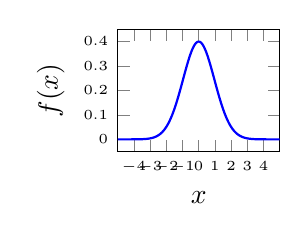
\begin{tikzpicture}
            \begin{axis}
                [
                    width=.3\textwidth,
                    axis lines = box,
                    xmin = -5, xmax = 5, ymin = -0.05, ymax = 0.45,
                    xlabel=\(x\), ylabel=\(f(x)\), samples=300,
                    yticklabel style = {font=\tiny},xticklabel style = {font=\tiny},
                    ytick={0,0.1,0.2,0.3,0.4},
                    yticklabels={0,0.1,0.2,0.3,0.4},
                    xtick={-4,-3,...,4}
                ]
                \addplot[domain=-5:5,thick,blue]{exp(-x^2 / 2) / (sqrt(2*pi) * (1 + x^2)^(1/30))};
            \end{axis}
        \end{tikzpicture}
        \caption{\(t\)分布の確率密度関数(概略)}
        \vspace{-.5cm}
    \end{wrapfigure}
    \noindent\textbf{帰無仮説\ \(H_0\):} 述べたい事柄を否定する仮説.帰無仮説を棄却することで,述べたい事柄を示す.今回は,視覚探索課題において「探索非対称性がないこと」が帰無仮説となる.\\ \\
    \textbf{対立仮説\ \(H_a\):} 述べたい事柄を支持するような仮説を立てる.\\ \\
    \textbf{\(t\)分布:} 正規分布に従う母集団の平均値,分散が不明である場合に利用する確率分布.標本数を\(n\),標本の平均値を\(\bar{X}\),不偏分散を\(s^2\)とし\(t\)分布は\eqref{equ:t分布}で定義される.\(n-1\)の値を自由度と呼び,\(t\)分布は自由度が増すほど正規分布に近くなる\cite[p.178\ -\ p.179]{応用解析と情報数学}.
    \begin{align}
        T & =\frac{\bar{X}-\mu}{\sqrt{s^2/n}}\label{equ:t分布}
    \end{align}
    \textbf{\(t\)検定:} \(t\)分布を利用する検定であり,ある値に対して,「ある値と異なる」ことが言えるかどうかを判断する検定方法.ここで用いるある値を\(t\)値と呼ぶ.今回は自由度を\(n\)としたときの\(t\)値を\eqref{equ:t値}に定め,両側検定を用いる.
    \begin{align}
        t(n) & = \frac{\textrm{回帰直線傾きの平均}}{\textrm{回帰直線傾きの標準誤差}}\label{equ:t値}
    \end{align}
    \textbf{有意確率\ \(p\):} 標本と帰無仮説が矛盾となる目安指標.\(p\)が小さいほど帰無仮説と標本が矛盾している.\\ \\
    \textbf{有意水準\ \(\alpha\):} 帰無仮説を棄却する基準となる値.有意確率\(p\)が有意水準を下回ったときに帰無仮説を棄却する.一般的には\(5\%\)か\(1\%\).今回の実験では,有意水準を\(5\%\)に設定する.
    \begin{itemize}
        \item \(p<\alpha\):有意差があり,帰無仮説が起こる確率は低く帰無仮説を棄却できる.つまり対立仮説を採択できる.
        \item \(p>\alpha\):有意差がなく,帰無仮説が起こる確率を無視できず,帰無仮説を棄却できない.
    \end{itemize}
    \textbf{標準誤差\(\textrm{SE}\):} 理論上の「標本平均の標準偏差」の大きさ.母集団の統計量の誤差を,標本から母集団の性質を推定した統計量の標準偏差として表したもので,\eqref{equ:標準誤差}で求める.
    \begin{align}
        \textrm{SE} & =\frac{\textrm{標準偏差}}{\sqrt{標本サイズ}}\label{equ:標準誤差}
    \end{align}
    \textbf{回帰直線:} 標本\((x_1,y_1),(x_2,y_2),\dots ,(x_n,y_n)\)に対して,
    \begin{align*}
        (y-y_1)^2+(y-y_2)^2+\dots +(y-y_n)^2
    \end{align*}
    を最小にするような直線\(y=ax+b\)を回帰直線という.\\
    \hfill\cite[p.168, p.187, p.200\ -\ p.205]{Pythonで学ぶあたらしい統計学の教科書}
\end{oframed}
\begin{multicols}{2}
    \begin{enumerate}
        \item 帰無仮説,対立仮説を立てる.
        \item 有意水準\(\alpha\)を設定する.今回は\(\alpha=0.05\).
        \item 検定統計量\(t\)値を求める.
        \item \(t\)値から有意確率\(p\)値を求める.
              \columnbreak
        \item 帰無仮説の棄却,採択の判断をする.
              \begin{itemize}
                  \item \(p<\alpha\):帰無仮説を棄却し,対立仮説を採択する.
                  \item \(p>\alpha\):帰無仮説を棄却しない.
              \end{itemize}
        \item \matlab を用いて,データの平均値と標準誤差の誤差線を出力する(\sref{src:14_01}).
    \end{enumerate}
\end{multicols}
今回の実験では,目標刺激が\texttt{C}と\texttt{CL}それぞれの目標刺激の有無に対して,探索非対称性がないことを帰無仮説とする.
当然,「探索非対称性があること」が対立仮説となる.データの集計にはGoogleスプレットシートを用いる.以下にGoogleスプレットシート上で用いる関数と,\tblref{tbl:データ集計}に集計方法を示す.
\begin{multicols}{2}
    \begin{description}
        \item[\texttt{AVERAGE(arg)}] 指定範囲の平均.
        \item[\texttt{VAR.S(arg)}] 指定範囲の不偏分散.
        \item[\texttt{STDEV.S(arg)}] 指定範囲の不偏標準偏差(標本標準偏差).
        \item[\texttt{COUNT(arg)}] 指定範囲の要素数.
        \item[\texttt{SQRT(arg)}] 引数の平方根.
        \item[\texttt{TDIST(arg1,arg2,arg3)}] \(p\)値を出力する.\texttt{arg1}に\(t\)値を,\texttt{arg2}に自由度\(\textrm{要素数}-1\)を,\texttt{arg3}に利用確率(今回は両側を利用するので\texttt{2}を代入)を格納する.
        \item[\texttt{SLOPE(arg1,arg2)}] 回帰直線の傾きを出力する.横座標に\texttt{arg1},縦座標に\texttt{arg2}を指定する.
    \end{description}
\end{multicols}
\input{table}
\footnotetext[1]{目標刺激の種類}
\(t\)値を\texttt{t = sAVE/sSD},\(p\)値を\texttt{p = TDIST(t,COUNT(range\_s)-1,2)}で求め,\tblref{tbl:データ集計}を\csv 形式で書き出す.\par
次に,\matlab でデータの平均値と標準誤差の誤差線を出力するスクリプトを記述する.\texttt{importdata}関数を用いて書き出した\csv を読み込む.
参加者番号を削除した後に,各統計量を求める.そのデータから平均値と標準誤差の誤差線を\texttt{err\_data}関数を用いて描画する.\par
最後に,読み込んだデータから回帰直線を求める.\tblref{tbl:データ集計}に示した方法を\matlab で再現し,\texttt{polyfit}関数と\texttt{slope}関数を用いて回帰直線の傾きと切片を求める.
参加者\(A\)のデータを散布図として,回帰直線と同時に描画する(\sref{src:14_02}).
\section{\result}
<実験1>で得られた実験参加者の平均値と標準誤差の誤差線を\figref{fig:平均値と誤差線},参加者\(A\)の結果に対する平均値と回帰直線を\figref{fig:平均値と回帰直線}に示す.
グラフ作成のもととなったデータを\tblref{tbl:探索時間},\tblref{tbl:回帰直線の傾き}に示す.参加者\(A\)は「参加者番号」列に明記した.\par
<実験2>で得られた,刺激対(\figref{fig:刺激対1},\figref{fig:刺激対2})の刺激数に対する探索時間を示したグラフを\figref{fig:刺激対の刺激数に対する探索時間}に示す.
\begin{figure}[H]
    \centering
    \begin{minipage}[b]{.49\textwidth}
        \centering
        \includegraphics[keepaspectratio,width=\textwidth]{../../Figures/14_01_graph.pdf}
        \caption{平均値と誤差線}
        \label{fig:平均値と誤差線}
    \end{minipage}
    \begin{minipage}[b]{.49\textwidth}
        \centering
        \includegraphics[keepaspectratio,width=\textwidth]{../../Figures/14_02_graph.pdf}
        \caption{参加者\(A\)の結果 散布図と回帰直線}
        \label{fig:平均値と回帰直線}
    \end{minipage}
\end{figure}
\begin{figure}[H]
    \centering
    \begin{minipage}[b]{.49\textwidth}
        \centering
        \includegraphics[keepaspectratio,width=\textwidth]{../../Figures/13_01_graph.pdf}
        \subcaption{刺激対1の刺激数に対する探索時間}
    \end{minipage}
    \begin{minipage}[b]{.49\textwidth}
        \centering
        \includegraphics[keepaspectratio,width=\textwidth]{../../Figures/13_02_graph.pdf}
        \subcaption{刺激対2の刺激数に対する探索時間}
    \end{minipage}
    \caption{<実験2>\ 各刺激対に対する探索時間}
    \label{fig:刺激対の刺激数に対する探索時間}
\end{figure}
有意水準\(5\%\)で対応のある\(t\)検定を行った結果,刺激対1の刺激\texttt{C}と\texttt{CL}の間で有意な差が認められた.
\begin{align}
    t(13) & =2.9150238 & p<0.05
\end{align}
\begin{table}[H]
    \centering
    \caption{探索時間}
    \label{tbl:探索時間}
    \fontsize{4}{7}\selectfont\ttfamily
    \input{../../14_DataAnalysisStatistical/result_table.tex}
\end{table}
\begin{table}[H]
    \centering
    \caption{回帰直線の傾き}
    \label{tbl:回帰直線の傾き}
    \fontsize{4}{7}\selectfont\ttfamily
    \begin{tabularx}{\textwidth}{|c|L|L|L|}
    \hline
    参加者番号 & \multicolumn{1}{c|}{目標刺激:円} & \multicolumn{1}{c|}{目標刺激:円+線} & \multicolumn{1}{c|}{差} \\
    \hline
    非表示   & 16.06991071                 & -1.435482143                  & 17.50539286            \\ \hline
    非表示   & 30.67642857                 & -13.39660714                  & 44.07303571            \\ \hline
    非表示   & 20.530625                   & 0.9915714286                  & 19.53905357            \\ \hline
    非表示   & 34.93921429                 & 16.5735                       & 18.36571429            \\ \hline
    非表示   & 30.43                       & -0.3654285714                 & 30.79542857            \\ \hline
    非表示   & 12.93405357                 & 1.196875                      & 11.73717857            \\ \hline
    非表示   & 16.70098214                 & -2.032321429                  & 18.73330357            \\ \hline
    非表示   & 28.13507143                 & -6.507107143                  & 34.64217857            \\ \hline
    非表示   & 19.35846429                 & -0.4041428571                 & 19.76260714            \\ \hline
    非表示   & 21.81151786                 & 2.088696429                   & 19.72282143            \\ \hline
    非表示   & 23.10467857                 & -4.515473214                  & 27.62015179            \\ \hline
    非表示   & 45.05892857                 & 6.948214286                   & 38.11071429            \\ \hline
    非表示   & 27.75228571                 & 6.975035714                   & 20.77725               \\ \hline
    非表示   & 18.57964286                 & 2.491964286                   & 16.08767857            \\ \hline\hline
    平均値   & 24.72012883                 & 0.6149496173                  & 24.10517921            \\ \hline
    不偏分散  & 75.39627981                 & 48.30711698                   & 88.89262924            \\ \hline
    標準偏差  & 8.683103121                 & 6.950332149                   & 9.428288776            \\ \hline
    標準誤差  & 2.320656924                 & 1.857554402                   & 2.519816167            \\ \hline
\end{tabularx}
\end{table}
\section{\consideration}
\paragraph{実験1}
結果より,目標刺激が\texttt{C}の場合,目標刺激数に伴って探索時間が増加していることがわかる.
それに対して目標刺激が\texttt{CL}の場合,刺激数に対する探索時間はおよそ一定である.
これらから\(t\)検定を用いて,両刺激(\texttt{C},\texttt{CL})には探索非対称性があると判断された.
この原因として,目標刺激が\texttt{CL}の探索に対してポップアウト現象が起きていることが考えられる.刺激\texttt{CL}は刺激\texttt{C}に一本の線を足した刺激なので,円刺激に比べて発見しやすい.
これに対して,目標刺激が\texttt{C}の探索では,刺激\texttt{CL}には\texttt{C}の「円」という要素を含んでいるので,ポップアウトは起きず,逐次探索になると考えられる.
\paragraph{実験2}
刺激対1に対する探索時間と,刺激対2に対する探索時間を比較する.刺激対1に比べて,刺激対2は探索時間の偏りは小さい.
刺激対2について,\texttt{Start}と\texttt{Diamond}の形状が似ており,判断の時間に差異が生まれないからであろう.
刺激対2の目標刺激がない場合は,刺激数に伴って探索時間が増加しており,
目標刺激がある場合は,目標刺激に限らず目標刺激数が8から16にかけて一定,または減少している.これは「探索非対称性」があるとは言えない.
\texttt{Star},\texttt{Diamond}の両刺激において,逐次探索でなくポップアウトが生じていると考えられる.
\section{\conclusion}
今回の実験では,視覚探索課題の心理物理実験をし,目標刺激と妨害刺激が交代しただけで探索時間が大きく異なる「探索非対称性」を検証した.
その原因となる「ポップアウト」が起きる刺激の条件と,「逐次探索」が起きる刺激の条件が明らかとなった.
さらに,統計的仮説検定を用いて,刺激\texttt{C}と刺激\texttt{CL}には探索時間に有意な差が認められ,探索非対称性を認められた.
